\section{1D Fourier Transform}
\subsection{Implementation}
\begin{figure} [!h]
    \centering
    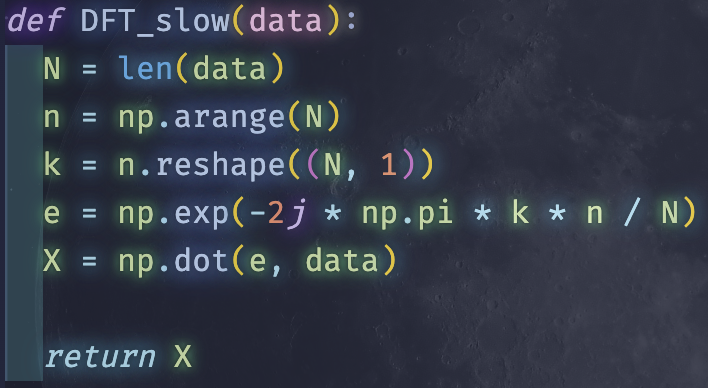
\includegraphics[width=1\textwidth]{img/code/1D.png}
    \caption{1D DFT Function}
\end{figure}


\newpage
\section{2D Fourier Transform}
\subsection{Implementation}
\begin{figure} [!h]
    \centering
    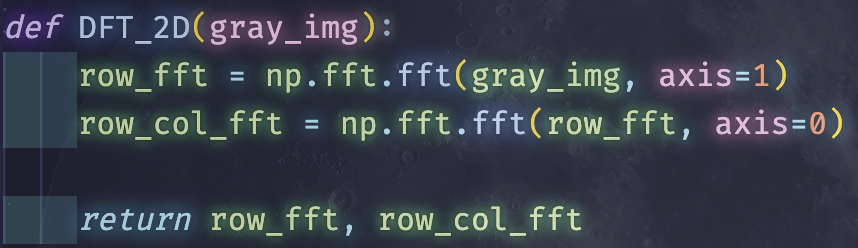
\includegraphics[width=1\textwidth]{img/code/2D.png}
    \caption{2D DFT Function}
\end{figure}

\subsection{Results}
\begin{figure} [!h]
    \centering
    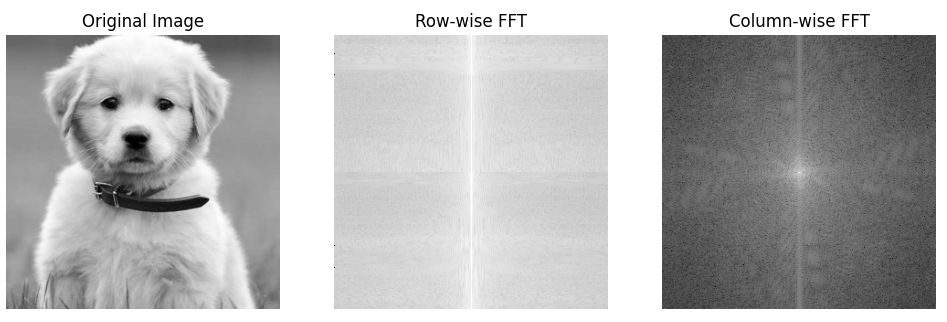
\includegraphics[width=1\textwidth]{img/DFT_2D.png}
    \caption{Output for 2D DFT Exercise}
\end{figure}


\newpage
\section{Frequency Removal Procedure}
\subsection{Implementation}
\begin{figure} [!h]
    \centering
    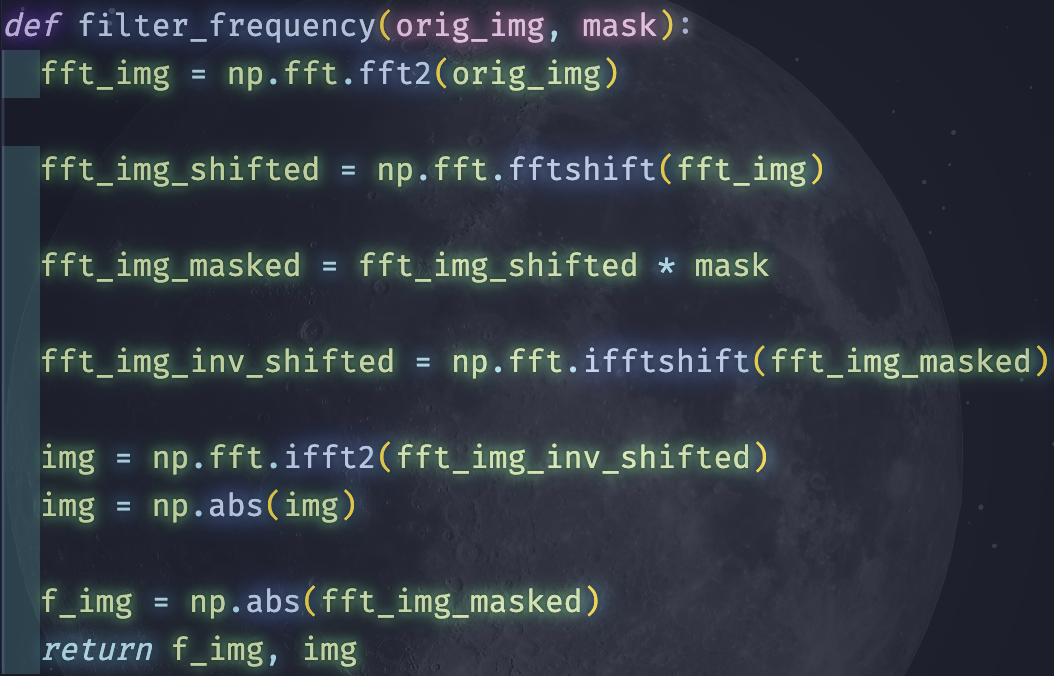
\includegraphics[width=0.75\textwidth]{img/code/freq.png}
    \caption{Frequency Removal Function}
\end{figure}

\subsection{Results}
\begin{figure} [!h]
    \centering
    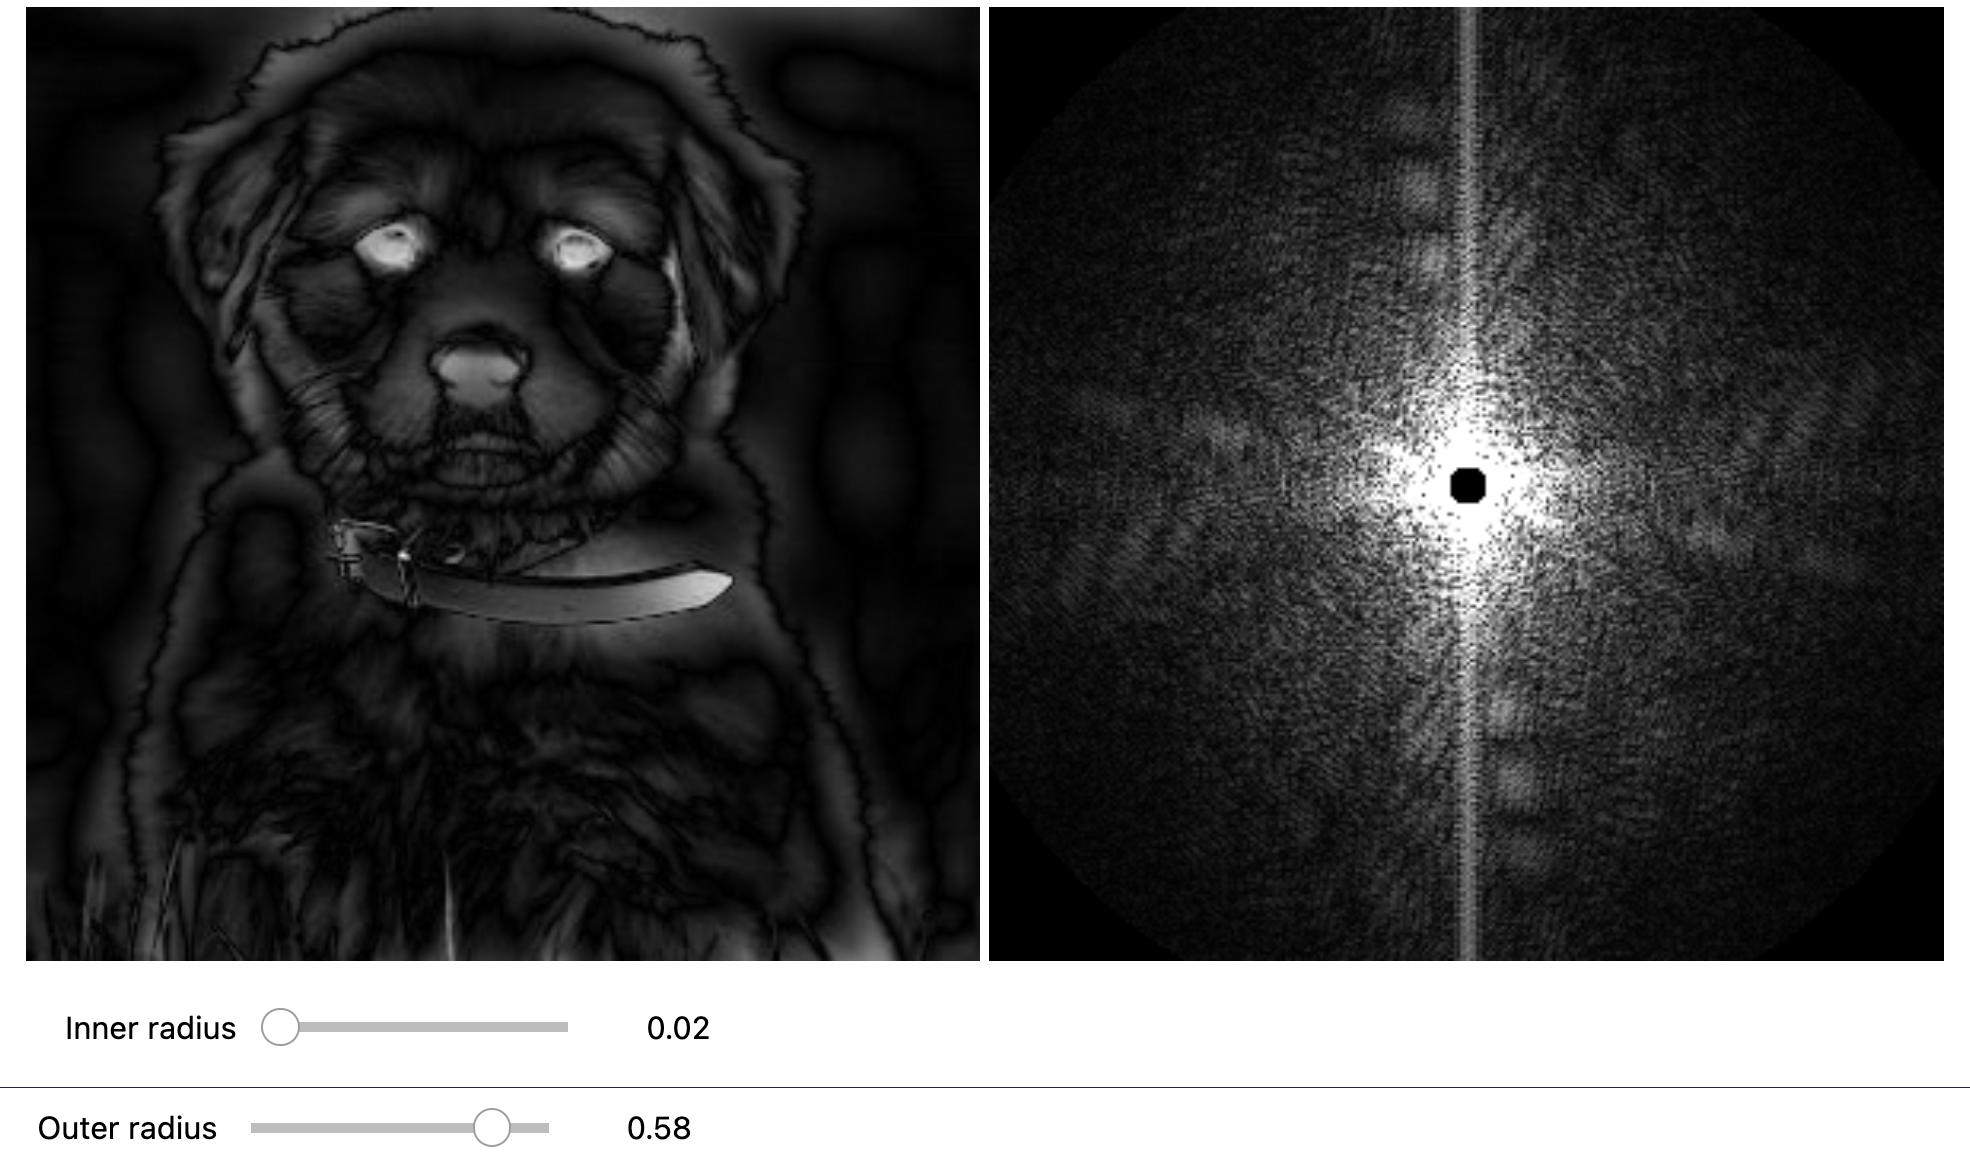
\includegraphics[width=0.75\textwidth]{img/freq.png}
    \caption{Output for Frequency Removal Exercise}
\end{figure}

\section{Hybrid Image}
\subsection{Implementation}
\begin{figure} [!h]
    \centering
    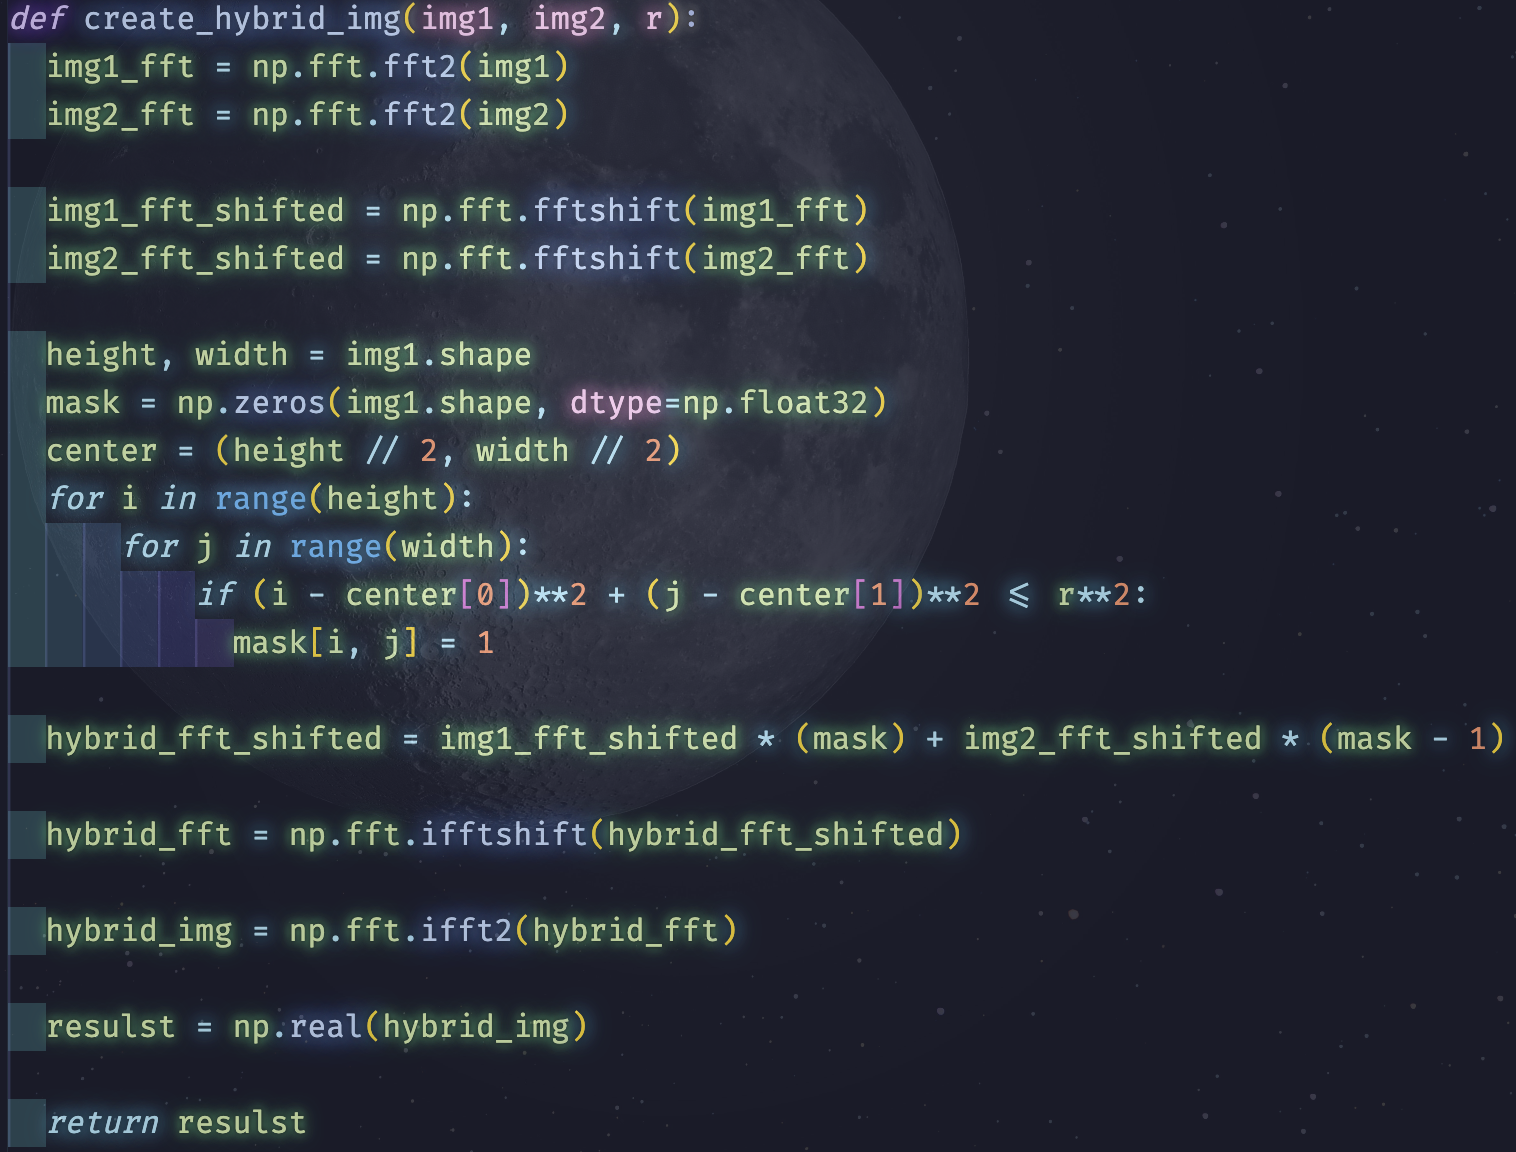
\includegraphics[width=0.95\textwidth]{img/code/hybrid.png}
    \caption{Hybrid Image Function}
\end{figure}

\subsection{Results}
\begin{figure} [!h]
    \centering
    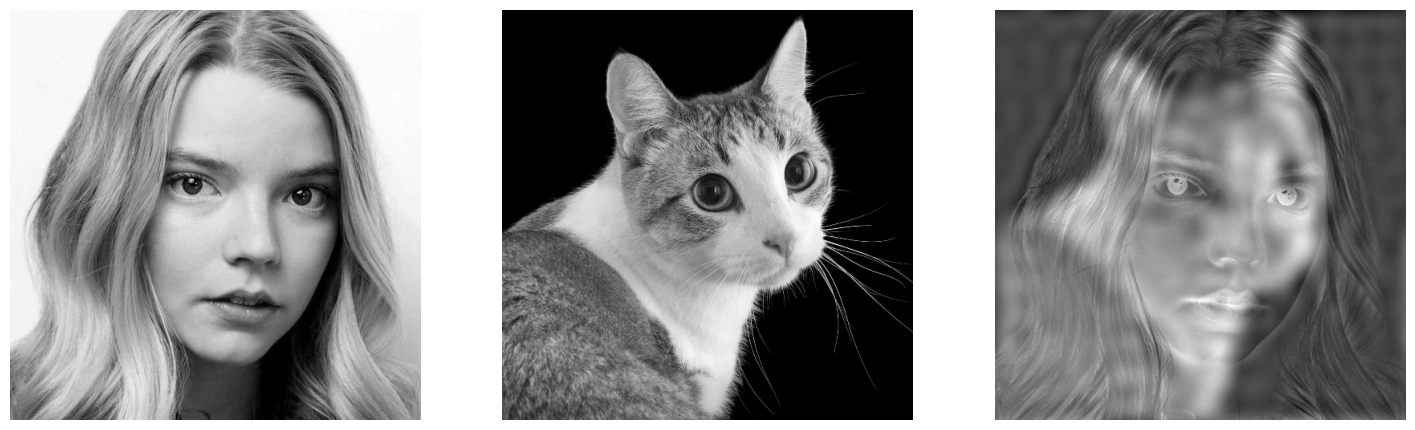
\includegraphics[width=1\textwidth]{img/hybrid.png}
    \caption{Hybrid image of a woman and a cat}
\end{figure}